\documentclass[]{article}
\usepackage{float}
\usepackage{graphicx}
\usepackage{blindtext}
\usepackage{longtable}
\usepackage{geometry}
 \geometry{
 a4paper,
 total={170mm,257mm},
 left=20mm,
 top=20mm,
 }

\title{Two Class PCA Analysis Report}
\author{Daniel Alimadadian}
\date{\today}

\begin{document}

\begin{titlepage}
    \maketitle
    \section*{Warnings}
    \section*{Data Summary}
\end{titlepage}

\section*{Principal Component Analysis (PCA) Summary}
    PCA analysis is performed using \texttt{sklearn} package version 1.1.2. \\
    Data scaling = \textbf{Standard}

    \begin{figure}[h!]
        \begin{center}
            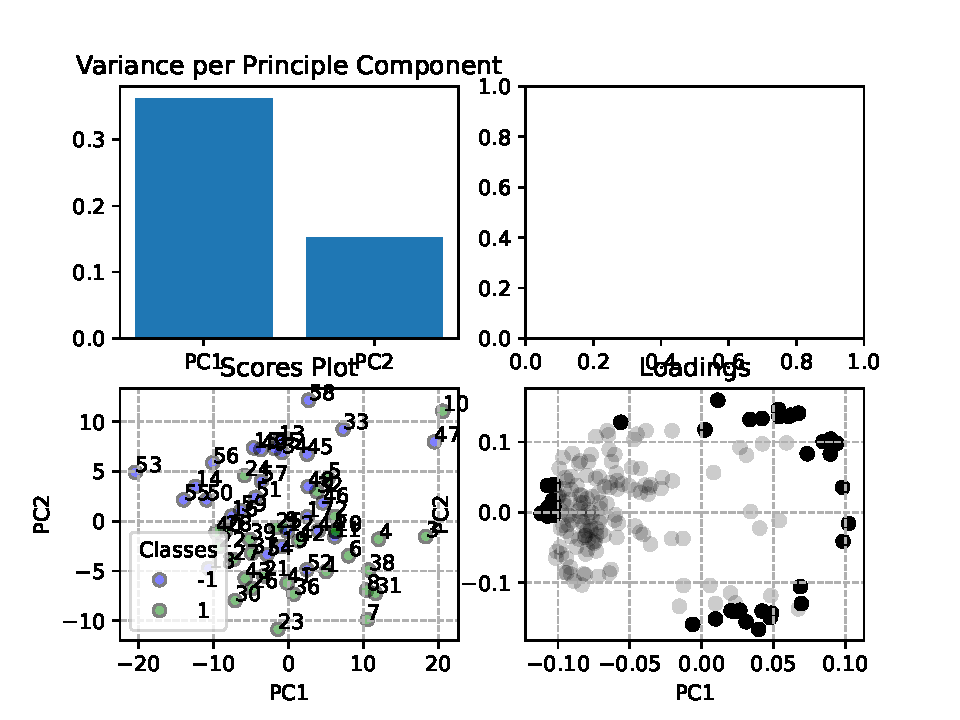
\includegraphics{summary_figs.pdf}    
        \end{center}
        \caption{PCA Summary}
    \end{figure}
    
\newpage

\section*{PC1 vs. PC2}
    Loadings selected from PC1: \textbf{20}. Loadings selected from PC2: \textbf{20} 

    \begin{figure}[h!]
        \begin{center}
            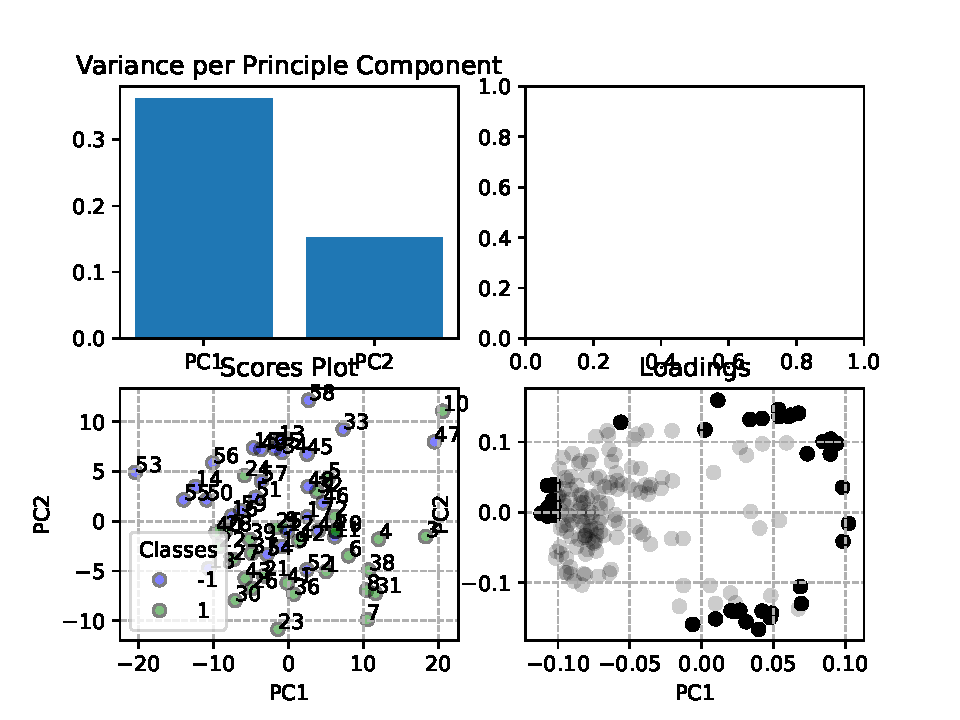
\includegraphics{summary_figs.pdf}
        \end{center}
        \caption{PCA scores plot. RRMS: n = \textbf{31}, SPMS: n = \textbf{28}}
    \end{figure}

\newpage

\section*{Ranked Loadings}

    \begin{figure}[h!]
        \begin{center}
            \includegraphics{ranked_loadings.pdf}
        \end{center}
        \caption{Ranked loadings plots. Top: (0.05, 0.95) quantiles
        represented by dashed red lines. Bottom: significant loadings are labelled.}
    \end{figure}

\newpage

\section*{Univariate Analysis}

    \begin{longtable}{ c c c c }
    \caption{Top loadings only. Student's t-test p-values < 0.05, 0.01, 0.001 are represented by *, ** and 
    *** respectively. NS: not significant.} \label{tab:long} \\
    \hline \\
        & p-value & Significance & Bonferroni \\
    \hline \\
    \endfirsthead
    \endhead
    X.1.14....1.16. & 0.0 & *** & 0.0\\
X.1.12....1.14. & 0.0 & *** & 3.7e-05\\
X.0.82....0.84. & 0.0 & *** & 5.8e-05\\
X.1.40....1.42. & 4e-06 & *** & 0.000791\\
X.1.22....1.24. & 4e-06 & *** & 0.000815\\
X.2.20....2.22. & 3.2e-05 & *** & 0.005989\\
X.0.84....0.86. & 9.9e-05 & *** & 0.01835\\
X.1.38....1.40. & 0.000128 & *** & 0.023682\\
X.5.24....5.26. & 0.000212 & *** & 0.039226\\
X.1.66....1.68. & 0.000514 & *** & 0.095074\\
X.1.74....1.76. & 0.000719 & *** & 0.132993\\
X.5.26....5.28. & 0.001566 & ** & 0.289645\\
X.1.98....2.00. & 0.001612 & ** & 0.298298\\
X.3.22....3.24. & 0.003884 & ** & 0.718623\\
X.2.70....2.72. & 0.010738 & * & 1.986581\\
X.5.28....5.30. & 0.014187 & * & 2.624533\\
X.2.52....2.54. & 0.022718 & * & 4.202833\\
X.0.86....0.88. & 0.024708 & * & 4.571052\\
X.1.72....1.74. & 0.028567 & * & 5.284857\\
X.2.66....2.68. & 0.036788 & * & 6.805745\\
X.1.26....1.28. & 0.038014 & * & 7.032682\\
X.2.32....2.34. & 0.046085 & * & 8.525671\\
X.1.36....1.38. & 0.064595 & NS & 11.950135\\
X.2.00....2.02. & 0.067999 & NS & 12.579817\\
X.1.70....1.72. & 0.09571 & NS & 17.706305\\
X.2.22....2.24. & 0.100395 & NS & 18.573158\\
X.1.34....1.36. & 0.102446 & NS & 18.952481\\
X.1.68....1.70. & 0.107744 & NS & 19.932595\\
X.1.56....1.58. & 0.133949 & NS & 24.780519\\
X.1.60....1.62. & 0.153084 & NS & 28.320536\\
X.5.34....5.36. & 0.274761 & NS & 50.830816\\
X.5.30....5.32. & 0.340391 & NS & 62.972353\\
X.1.58....1.60. & 0.348753 & NS & 64.519324\\
X.5.32....5.34. & 0.37547 & NS & 69.46195\\
X.3.98....4.00. & 0.423476 & NS & 78.343105\\
X.2.24....2.26. & 0.437745 & NS & 80.982825\\
X.0.88....0.90. & 0.509072 & NS & 94.178272\\
X.3.96....3.98. & 0.666832 & NS & 123.363845\\
X.1.30....1.32. & 0.909419 & NS & 168.242602\\
X.1.28....1.30. & 0.965595 & NS & 178.635141   
    \end{longtable}

    \newpage

    \begin{longtable}{ c c c c }
    \caption{All features. Student's t-test p-values < 0.05, 0.01, 0.001 are represented by *, ** and 
    *** respectively. NS: not significant.} \label{tab:long} \\
    \hline \\
        & p-value & Significance & Bonferroni \\
    \hline \\
    \endfirsthead
    \endhead
    X.0.80....0.82. & 0.0 & *** & 0.0\\
X.1.14....1.16. & 0.0 & *** & 0.0\\
X.2.16....2.18. & 0.0 & *** & 5e-06\\
X.2.18....2.20. & 0.0 & *** & 6e-06\\
X.1.12....1.14. & 0.0 & *** & 3.7e-05\\
X.0.82....0.84. & 0.0 & *** & 5.8e-05\\
X.1.76....1.78. & 0.0 & *** & 6.5e-05\\
X.1.42....1.44. & 1e-06 & *** & 0.000199\\
X.1.16....1.18. & 1e-06 & *** & 0.000203\\
X.2.82....2.84. & 4e-06 & *** & 0.000738\\
X.1.40....1.42. & 4e-06 & *** & 0.000791\\
X.1.22....1.24. & 4e-06 & *** & 0.000815\\
X.1.64....1.66. & 1e-05 & *** & 0.001861\\
X.1.44....1.46. & 1.5e-05 & *** & 0.002724\\
X.2.20....2.22. & 3.2e-05 & *** & 0.005989\\
X.7.82....7.84. & 5.4e-05 & *** & 0.010047\\
X.2.10....2.12. & 5.8e-05 & *** & 0.010639\\
X.1.20....1.22. & 8.2e-05 & *** & 0.015088\\
X.2.48....2.50. & 8.4e-05 & *** & 0.015485\\
X.0.84....0.86. & 9.9e-05 & *** & 0.01835\\
X.2.36....2.38. & 0.000111 & *** & 0.020484\\
X.2.84....2.86. & 0.000124 & *** & 0.022979\\
X.1.38....1.40. & 0.000128 & *** & 0.023682\\
X.2.34....2.36. & 0.00018 & *** & 0.033309\\
X.1.62....1.64. & 0.000185 & *** & 0.034261\\
X.2.08....2.10. & 0.00019 & *** & 0.035206\\
X.5.24....5.26. & 0.000212 & *** & 0.039226\\
X.1.24....1.26. & 0.000244 & *** & 0.045225\\
X.2.80....2.82. & 0.000393 & *** & 0.07267\\
X.1.66....1.68. & 0.000514 & *** & 0.095074\\
X.1.74....1.76. & 0.000719 & *** & 0.132993\\
X.2.64....2.66. & 0.001087 & ** & 0.201041\\
X.3.80....3.82. & 0.001192 & ** & 0.220474\\
X.2.50....2.52. & 0.001278 & ** & 0.236448\\
X.1.18....1.20. & 0.001499 & ** & 0.277336\\
X.5.26....5.28. & 0.001566 & ** & 0.289645\\
X.1.98....2.00. & 0.001612 & ** & 0.298298\\
X.3.20....3.22. & 0.001689 & ** & 0.312531\\
X.3.78....3.80. & 0.002233 & ** & 0.413042\\
X.2.06....2.08. & 0.002698 & ** & 0.499086\\
X.7.66....7.68. & 0.003367 & ** & 0.622849\\
X.3.22....3.24. & 0.003884 & ** & 0.718623\\
X.2.54....2.56. & 0.003987 & ** & 0.737574\\
X.3.62....3.64. & 0.004424 & ** & 0.818434\\
X.1.46....1.48. & 0.0058 & ** & 1.072987\\
X.3.12....3.14. & 0.007126 & ** & 1.31822\\
X.3.92....3.94. & 0.007183 & ** & 1.328947\\
X.3.36....3.38. & 0.007957 & ** & 1.471999\\
X.3.32....3.34. & 0.008311 & ** & 1.537579\\
X.3.52....3.54. & 0.008508 & ** & 1.574026\\
X.2.04....2.06. & 0.009164 & ** & 1.695274\\
X.1.52....1.54. & 0.009215 & ** & 1.704842\\
X.2.70....2.72. & 0.010738 & * & 1.986581\\
X.3.50....3.52. & 0.011526 & * & 2.132398\\
X.1.96....1.98. & 0.013348 & * & 2.469468\\
X.5.28....5.30. & 0.014187 & * & 2.624533\\
X.1.88....1.90. & 0.016543 & * & 3.060454\\
X.3.38....3.40. & 0.017334 & * & 3.20679\\
X.2.14....2.16. & 0.017382 & * & 3.215745\\
X.3.88....3.90. & 0.020557 & * & 3.80303\\
X.1.54....1.56. & 0.02128 & * & 3.93673\\
X.2.52....2.54. & 0.022718 & * & 4.202833\\
X.3.16....3.18. & 0.022895 & * & 4.235654\\
X.2.86....2.88. & 0.024336 & * & 4.502164\\
X.0.86....0.88. & 0.024708 & * & 4.571052\\
X.1.48....1.50. & 0.02687 & * & 4.970917\\
X.3.30....3.32. & 0.028526 & * & 5.277219\\
X.1.72....1.74. & 0.028567 & * & 5.284857\\
X.1.92....1.94. & 0.029038 & * & 5.372102\\
X.5.22....5.24. & 0.032077 & * & 5.934208\\
X.3.44....3.46. & 0.03313 & * & 6.128966\\
X.3.76....3.78. & 0.036122 & * & 6.682542\\
X.2.66....2.68. & 0.036788 & * & 6.805745\\
X.3.86....3.88. & 0.037231 & * & 6.887763\\
X.1.26....1.28. & 0.038014 & * & 7.032682\\
X.3.82....3.84. & 0.038944 & * & 7.2046\\
X.3.90....3.92. & 0.040395 & * & 7.473145\\
X.3.70....3.72. & 0.041926 & * & 7.756265\\
X.2.32....2.34. & 0.046085 & * & 8.525671\\
X.7.34....7.36. & 0.047347 & * & 8.759171\\
X.2.90....2.92. & 0.048594 & * & 8.989857\\
X.3.46....3.48. & 0.053842 & NS & 9.960819\\
X.7.80....7.82. & 0.055891 & NS & 10.33978\\
X.7.08....7.10. & 0.056102 & NS & 10.37888\\
X.3.84....3.86. & 0.057616 & NS & 10.658926\\
X.3.60....3.62. & 0.058245 & NS & 10.775417\\
X.2.38....2.40. & 0.062129 & NS & 11.493951\\
X.1.36....1.38. & 0.064595 & NS & 11.950135\\
X.3.54....3.56. & 0.066826 & NS & 12.362756\\
X.2.00....2.02. & 0.067999 & NS & 12.579817\\
X.7.30....7.32. & 0.071854 & NS & 13.292916\\
X.3.72....3.74. & 0.072441 & NS & 13.401605\\
X.3.40....3.42. & 0.07306 & NS & 13.51616\\
X.7.24....7.26. & 0.073096 & NS & 13.522687\\
X.7.04....7.06. & 0.074519 & NS & 13.78603\\
X.3.56....3.58. & 0.080197 & NS & 14.83636\\
X.1.50....1.52. & 0.082146 & NS & 15.196992\\
X.2.94....2.96. & 0.087142 & NS & 16.121337\\
X.2.96....2.98. & 0.090002 & NS & 16.650456\\
X.1.00....1.02. & 0.090074 & NS & 16.663614\\
X.3.48....3.50. & 0.092312 & NS & 17.077693\\
X.0.92....0.94. & 0.095583 & NS & 17.682925\\
X.1.70....1.72. & 0.09571 & NS & 17.706305\\
X.3.42....3.44. & 0.096861 & NS & 17.919224\\
X.2.22....2.24. & 0.100395 & NS & 18.573158\\
X.1.34....1.36. & 0.102446 & NS & 18.952481\\
X.7.10....7.12. & 0.104584 & NS & 19.347963\\
X.3.58....3.60. & 0.107275 & NS & 19.84584\\
X.1.68....1.70. & 0.107744 & NS & 19.932595\\
X.0.94....0.96. & 0.116026 & NS & 21.464856\\
X.7.06....7.08. & 0.120252 & NS & 22.246565\\
X.3.64....3.66. & 0.126732 & NS & 23.445354\\
X.1.56....1.58. & 0.133949 & NS & 24.780519\\
X.3.00....3.02. & 0.136565 & NS & 25.264444\\
X.3.04....3.06. & 0.140817 & NS & 26.051123\\
X.1.60....1.62. & 0.153084 & NS & 28.320536\\
X.7.78....7.80. & 0.156449 & NS & 28.943037\\
X.3.74....3.76. & 0.16136 & NS & 29.851621\\
X.7.42....7.44. & 0.17012 & NS & 31.472235\\
X.2.42....2.44. & 0.172529 & NS & 31.917828\\
X.2.78....2.80. & 0.173896 & NS & 32.170672\\
X.4.06....4.08. & 0.174079 & NS & 32.204617\\
X.2.28....2.30. & 0.189019 & NS & 34.968439\\
X.2.46....2.48. & 0.196837 & NS & 36.414882\\
X.3.68....3.70. & 0.19873 & NS & 36.765031\\
X.2.12....2.14. & 0.215956 & NS & 39.951769\\
X.7.36....7.38. & 0.216336 & NS & 40.022225\\
X.6.88....6.90. & 0.225121 & NS & 41.647338\\
X.3.94....3.96. & 0.225978 & NS & 41.805916\\
X.2.40....2.42. & 0.238127 & NS & 44.053558\\
X.7.14....7.16. & 0.248154 & NS & 45.908495\\
X.2.98....3.00. & 0.253306 & NS & 46.86166\\
X.5.34....5.36. & 0.274761 & NS & 50.830816\\
X.3.10....3.12. & 0.277202 & NS & 51.28238\\
X.4.08....4.10. & 0.277907 & NS & 51.412815\\
X.2.92....2.94. & 0.288901 & NS & 53.446644\\
X.2.26....2.28. & 0.327304 & NS & 60.551182\\
X.2.02....2.04. & 0.327952 & NS & 60.671165\\
X.5.30....5.32. & 0.340391 & NS & 62.972353\\
X.1.58....1.60. & 0.348753 & NS & 64.519324\\
X.7.18....7.20. & 0.364698 & NS & 67.469056\\
X.5.32....5.34. & 0.37547 & NS & 69.46195\\
X.3.66....3.68. & 0.392902 & NS & 72.686827\\
X.1.94....1.96. & 0.398497 & NS & 73.721998\\
X.6.70....6.72. & 0.398925 & NS & 73.801157\\
X.2.30....2.32. & 0.420527 & NS & 77.797488\\
X.1.90....1.92. & 0.421478 & NS & 77.973369\\
X.3.98....4.00. & 0.423476 & NS & 78.343105\\
X.2.24....2.26. & 0.437745 & NS & 80.982825\\
X.7.40....7.42. & 0.439363 & NS & 81.282224\\
X.1.32....1.34. & 0.474551 & NS & 87.791939\\
X.4.10....4.12. & 0.487235 & NS & 90.138413\\
X.0.88....0.90. & 0.509072 & NS & 94.178272\\
X.0.90....0.92. & 0.52763 & NS & 97.611542\\
X.0.98....1.00. & 0.530172 & NS & 98.081857\\
X.2.76....2.78. & 0.540494 & NS & 99.991376\\
X.7.32....7.34. & 0.552406 & NS & 102.19505\\
X.3.28....3.30. & 0.586326 & NS & 108.470326\\
X.2.68....2.70. & 0.587397 & NS & 108.668381\\
X.4.00....4.02. & 0.59328 & NS & 109.756721\\
X.0.96....0.98. & 0.594713 & NS & 110.021939\\
X.3.34....3.36. & 0.600971 & NS & 111.179727\\
X.4.02....4.04. & 0.613818 & NS & 113.556288\\
X.3.26....3.28. & 0.626795 & NS & 115.957137\\
X.1.02....1.04. & 0.665433 & NS & 123.105126\\
X.3.96....3.98. & 0.666832 & NS & 123.363845\\
X.6.90....6.92. & 0.671236 & NS & 124.178664\\
X.2.44....2.46. & 0.683117 & NS & 126.376728\\
X.4.04....4.06. & 0.738955 & NS & 136.70675\\
X.4.14....4.16. & 0.750672 & NS & 138.874263\\
X.7.22....7.24. & 0.777715 & NS & 143.877323\\
X.3.06....3.08. & 0.82067 & NS & 151.823958\\
X.7.38....7.40. & 0.838504 & NS & 155.123319\\
X.3.24....3.26. & 0.881334 & NS & 163.046824\\
X.3.08....3.10. & 0.89879 & NS & 166.27623\\
X.1.30....1.32. & 0.909419 & NS & 168.242602\\
X.1.04....1.06. & 0.926574 & NS & 171.416256\\
X.3.18....3.20. & 0.927192 & NS & 171.530524\\
X.4.16....4.17. & 0.935577 & NS & 173.081699\\
X.3.02....3.04. & 0.952283 & NS & 176.172429\\
X.4.12....4.14. & 0.9524 & NS & 176.193935\\
X.2.74....2.76. & 0.952835 & NS & 176.274542\\
X.2.88....2.90. & 0.959402 & NS & 177.489417\\
X.1.28....1.30. & 0.965595 & NS & 178.635141\\
X.2.72....2.74. & 0.968797 & NS & 179.227445   
    \end{longtable}

\end{document}